\documentclass[twoside,english]{uiofysmaster/uiofysmaster}

\usepackage[toc,titletoc,title,page]{appendix} %to add appendices (and have them in toc)
%\usepackage{mhchem} %latex chemistry symbols
\usepackage{blindtext} %to fill in dummy text
%\usepackage{cite} %to have multiple citations in one \cite{key1,key2,..} -do not use with natbib!!
\usepackage{tcolorbox} %to have boxes w color around text and math mode
\usepackage{enumitem} %to reduce vertical spacing in enumerate
\usepackage{tabu} % to set tables to page width
%\usepackage{aas_macros}

\usepackage[sort&compress,square,comma,numbers]{natbib} %to use \citet, now mixed with [nr]
\usepackage[nottoc]{tocbibind}

%chapterlayout


\interfootnotelinepenalty=10000 % to force footnotes to NOT run over to the next page

%---
% to reduce space around table of contents (to fit everything into one page): 
\usepackage{tocloft}
\setlength{\cftbeforetoctitleskip}{0pt}
\setlength{\cftaftertoctitleskip}{0pt}
%---

\usepackage{epigraph}
\setlength\epigraphwidth{11cm}
\setlength\epigraphrule{0pt}

%---
\newcommand{\Cu}{${}^{64}$Cu} % making it faster to write Os192
\newcommand{\Osreac}{${}^{192}$Os$(\alpha$, $\alpha ' \gamma){}^{192}$Os}
\newcommand{\Osreacto}{${}^{191}$Os$(n$, $\gamma){}^{192}$Os}
\newcommand{\betadecay}{$\beta$-decay} % making it faster to write 
\newcommand{\bref}{B$^2$FH} % making it faster to write 
\newcommand{\gsf}{$\gamma$-strength function}
\newcommand{\ga}{$\gamma$}

%---
% modifying color in code listings and some style
\usepackage{color}
 
%\definecolor{codegreen}{rgb}{0,0.6,0} % too flashy
\definecolor{codegreen}{rgb}{0.0, 0.42, 0.24} % less flashy so comments not take all attention
\definecolor{codegray}{rgb}{0.5,0.5,0.5}
\definecolor{codepurple}{rgb}{0.58,0,0.82}
%\definecolor{codepurple}{rgb}{1.0, 0.0, 0.22} %carminered, could try it 
%\definecolor{backcolour}{rgb}{0.95,0.95,0.92} % original suggestion
\definecolor{backcolour}{rgb}{0.94, 0.97, 1.0}% aliceblue, not so flashy and not as ugly
 
\lstdefinestyle{mystyle}{
    backgroundcolor=\color{backcolour},   
    commentstyle=\color{codegreen},
    %commentstyle=\color{codegray},    
    keywordstyle=\color{magenta},
    numberstyle=\tiny\color{codegray},
    stringstyle=\color{codepurple},
    basicstyle=\footnotesize,
    breakatwhitespace=false,         
    breaklines=true,                 
    captionpos=b,                    
    keepspaces=true,                 
    %numbers=left,     %removing line numbers in the code snippets               
    %numbersep=5pt,                  
    showspaces=false,                
    showstringspaces=false,
    showtabs=false,                  
    tabsize=2,
    %float=tp,
    %floatplacement=tbp
}
 
\lstset{style=mystyle}
\renewcommand{\lstlistingname}{Code}
%---

%---
% new tcolorbox environment
% #1: tcolorbox options
% #2: color
% #3: box title
\newtcolorbox{mybox}[3][]
{
  colframe = #2!25,
  colback  = #2!10,
  coltitle = #2!20!black,  
  title    = #3,
  #1,
}

%---


%\bibliography{references}

\author{Nora Irene Jensen Pettersen}
\title{Cross-section meassurements for  $^{nat}Zn(n,p)64,67Cu$ reaction
%\title{Nuclear impact on astronomical processes: a first experimental constraint on the s-process $^{191}$Os$(n,\gamma)$ reaction rate %for the s-process in AGB stars
%\title{Nuclear impact on astronomical processes: benchmarking indirect measurements of s-process reaction rates for \Os 
}
\date{May 2020}
 
% ----------------------------------------------------------------------------------------------------------------------
% ----------------------------------------------------------------------------------------------------------------------
%Equations
%
%The command \eqref{} works exactly like \ref{}, but it adds parantheses to a plain number.
%
%Figures and tables
%
%\autoref{} is a usefull command when refering to to figures and tables. The command creates a reference with additional text corresponding to the target's type. For example, the command \autoref{fig:myfigure} would create a hyperlink to the \label{fig:myfigure} command, wherever it is. Assuming that this label is pointing to a figure, the hyperlink would contain the text "Figure 1.1", or similar.

%Two basic citation commands, \citet and \citep for textual and parenthetical citations, respectively. …
%\citet{jon90} --> Jones et al. (1990)
%\citep{jon90} --> (Jones et al., 1990)
%\citet*{jon90} --> Jones, Baker, and Williams (1990)
%\citep*{jon90} --> (Jones, Baker, and Williams, 1990)


\begin{document}

% set space around equations
\setlength{\belowdisplayskip}{12pt} \setlength{\belowdisplayshortskip}{12pt}
\setlength{\abovedisplayskip}{12pt} \setlength{\abovedisplayshortskip}{12pt}

\maketitle

%Centering the front page, see: https://github.com/ComputationalPhysics/uiofysmaster

\begin{abstract}
%An abstract summarizes, usually in one paragraph of 300 words or less, the major aspects of the entire paper in a prescribed sequence that includes: 1) the overall purpose of the study and the research problem(s) you investigated; 2) the basic design of the study; 3) major findings or trends found as a result of your analysis; and, 4) a brief summary of your interpretations and conclusions.


%However, it is difficult to conclude on the significance of the result.


\end{abstract}

\begin{dedication}
  %Til min kjære
  hola
  \\\vspace{12pt}
  %This is in dedication to 
This is for me.     % To my dear oppvaskmaskin. Du vet hvem du er. 
    
  

  
\end{dedication}

\begin{acknowledgements}
THANKS


Thank you grandmother, for being my safe place, even now. 
  \vspace{1.5cm}
  
  \noindent\textit{Nora Irene Jensen Pettersen}\\
  
  \noindent DATO
  
\end{acknowledgements}

\tableofcontents


% ----------------------------------------------------------------------------------------------------------------------
% ----------------------------------------------------------------------------------------------------------------------

\chapter{Introduction}

%heller i konklusjonen? eller?
\epigraph{\itshape ``Count only the good days."}{--- \textup{ Irene Jensen}, Ahus 2017}
 
% Abbe G. Lemaitre (Observatory, Louvain), Nature 1931


%Cancer. It can happen to us all, whether we like it or not. We all know someone or know someone who knows someone with cancer or had died of cancer. It sucks. But what if. What if there was a way to get rid of it? A tumor inside you, that grows without you knowing it. It can take years without you knowing it is there, and when you feel it, it might be too late. With regular radiation you will have that risk of radiate healthy cells and damage them, and over time they can become new cancer cells which can kill you all over again. That is why I want to look into this kind of radiation, where you radiate from the inside and out. Where you don’t damage to many healthy cells but only the bad ones. This type of radiation can reach places in the body where regular radiation will not, in the brain and deep under the skin. A patient with brain tumor can not be radiated because that will also damage other part of the brain that the person needs, so why not send the radioactive molecule into the tumor itselfs? I would.







%SEC: a short history lesson and intro to astrophys/cosmo/nuc astro
%\section*{A short astronomical history lesson} 
\paragraph{A short introduction to nuclear medicine} \mbox{}
%\paragraph{A short astronomical history lesson} \mbox{}




% ----------------------------------------------------------------------------------------------------------------------
% ----------------------------------------------------------------------------------------------------------------------

\chapter{Theory}
\label{ch: beyond}

\epigraph{\itshape quote}{--- \textup{by}, }
 


\section{Background of Nuclear medicine}
\label{sec:Background}

- why does it work \\
- how how we been doing nuclear medicine	\\
- what isotopes are we currently using in clinics\\
- problems with is\\
- my work\\

\section{Characteristics of medical radionuclides}
\noindent
\\
Radionuclides for therapeutic and diagnostic use have three principle factors that affect the ability for it to preform as a medical isotope in medicine\cite{invivo}, biological-, physical-, and chemical properties.\\
The biological and chemical feature involves the stability in a living organism, biological half-life, toxicity, tissue targeting and retention of radioactivity in the tumor\cite{Yeong}.
The physical characteristics include physical half-life, energy of the radiation, purity of the radionuclide, type of emission, daughter product(s) and method of production\cite{Yeong}. \\
\\\\
In this section, a book by Krane\cite{Krane} is used to describe the general nuclear reactions.\\

\subsection{Half-life}
The physical half-life, $t_{1/2}$, of a radioactive substance is the time it takes for a given amount to be reduced by half as a consequence of its decay and is described by the formula $$N(t) = N_0e^{-\lambda} t$$ 
where $N_0$ is the amount of initial substance, N(t) is then how much there is left after time, t, and $\lambda$ is the decay constant. This equation can be solved and the half-life of the decaying quantity is then given as $$t_{1/2} = \frac{ln2}{\lambda}$$ \\
\\
When a radioactive pharmaceutical gets injected into a human body, the biological half-life is important. It is the time it takes for a living body to reduce a biological substance by half through its biological processes. Therefore, when a radiopharmaceutical is produced to be used in a patients body, this is something that has to be considered carefully. It should be long enough to do a procedure, but short enough to not damage unnecessary healthy tissue. \\
\\
In diagnostic, the half-life should only be a few hours. From when the radioisotope is produced it starts to decay, and it is important that the half-life is long enough such that it can be used. If a patient is taking a PET-scan, depending on the radionuclide, a procedure using $^{18}F$ usually takes 30-60 minutes to execute. Therefore, the radiopharmaceutical have to have a half-life longer than it takes from production of the radioactive substance to the end of the procedure.
\\
\\
For a therapeutic isotope, it should have a half-life of approximately a few days. It should be long enough to deliver the right amount of dose to the area of interest. But the most important factor is the effective half-life, that is both physical and biological half-life within a patients organ\cite{Yeong}. The physical half-life is well known, but the biological half-life is dependent on several things, like what kind of tracer is being used, metabolism, uptake and how the pharmaceutical leaves the body\cite{Yeong}.\\
It depends on the uptake mechanism, type of tumor and method of administration\cite{Yeong} on what kind of tracer and isotope that should be used. If the patient has a low uptake, the physical half-life should be longer such that it will not emit radiation before it has reached the tumor, but not too long such that it sends out radiation on its way out of the body. 
\\
\\
Travel time is also a factor when choosing an isotope. Based on the physical half-life, some hospitals can produce some radioisotopes themselves. If they have a cyclotron in the hospital they can produce some isotopes, such as $^{18}F$ with half-life of 109 minutes, that is used in PET scans. In those cases the half-life can be shorter than if it has to be transported to another part of the county. \\
\\
\subsection{Stopping power}
When a charged particle penetrates an absorbing medium it will slowly slow down due to energy loss, the parameter that describes that is called stopping power. There are two known cases of stopping power\cite{Nuclear_medicine}, collision, $S_{col}$, and radiative, $S_{rad}$, stopping power. $S_{col}$ is a result from charged particles interaction with orbital electron of the material while $S_{rad}$ is when the charged particle interact with the nuclei in the material. The total stopping power is $S_{tot} = S_{col} + S_{rad}$ \\
\\
When a heavy charged particle looses its energy it is mainly by ionization where the mean energy loss is often described by Bethe-Block equation\cite{nuclearchem}.
\begin{equation}
    \frac{dE}{dX} = kz^2 \frac{Z}{A} \frac{1}{\beta^2} \left[ \frac{1}{2}ln \frac{2m_e c^2 \beta^2 \gamma^2 T_{max}}{I^2} - \beta^2 - \frac{\delta}{2} - \frac{C}{Z} \right]
\end{equation}
\begin{tabular}{l|l}
     K = constant & z = particle charge  \\
     Z = Atomic number & A = Mass number \\
     $\beta$ = v/c = Relative speed of the incident particle & $m_e c^2$ = Electron rest mass x $c^2$ \\
     $\gamma$ = Relativistic factor & $T_{max}$ = max kinetic energy given to a electron \\
     I = Mean excitation energy & $\delta$ = Density effect correction \\
     C/Z = shell correction & c = speed of light\\
\end{tabular}
\\
\\
The Bethe-Block equation can look different for different energies, electrons and secondary electrons. It reproduces the data experimentally in the energy region between a few MeV up to a few GeV\cite{nuclearchem} \\
\textcolor{red}{ The energy loss for electrons alters logarithmic with ionization loss and Z varies linearly, but the radiation loss increases linearly with the energy and almost quadratically with Z. Therefore, the stopping power for electron is most important for low energy electrons}\cite{nuclearchem}.\\
\\
For heavy charged particle with high energy there will be radiation losses that must be taken into account. The atomic shell-effect is something that happens at low energies.\cite{nuclearchem}\\
For intermediate energies, the Bethe-Block can be simplified to a point where the stopping power only is dependent by the charge and velocity of the incoming particle, the atomic mass number of the medium and the ionization potential\cite{nuclearchem}.\\
\\
Electrons can lose energy by Bremsstrahlung and by ionization. At high energies where a particle travels faster than the speed of light in a medium, Cherenkov radiation happens. This is an important phenomena but the energy loss in this process is small\cite{nuclearchem}.\\
\\
Even though the majority of the energy loss for electron is by collisions, the emission of bremsstrahlung photons is also important. When an electron is traveling close to an atomic nucleus it can decelerate due to the Coulomb field of the nucleus and atomic electrons. When this happens, the electron will transfer energy to a photon that gets emitted. When the kinetic energy of the electron increases the yield of bremsstrahlung increases.
\\
\\
When it comes to photons, the beam intensity I(x) will decrease with \begin{equation}
    I(x) = I_0e^{-\mu x}
\end{equation}
\noindent
where $\mu$ is the attenuation coefficient and are dependent of the energy h$\nu$ of the photon and the atomic number Z of the absorber\cite{Nuclear_medicine}. $I_0$ is the initial intensity of the beam at depth in medium where x = 0.\\
\\
Photons will also interact with a medium through photoelectric effect, Compton scattering and pair production, these are briefly discussed in section 2.1.3 under $\gamma$ and X-rays.\\
\\
\\
\noindent
\textbf{LET}\\
For therapy, the biological effect depends on how the isotopes decay, and how it distributes its energy to the surrounding medium. High linear energy transfer (LET) will concentrate the deposited energy to a small area near its tracks, as a result the biological damage is grater and there will be more damage to the DNA and other cellular structure. LET is closely related to the linear energy loss $\frac{dE}{dx}$ except that LET does not include radiative losses of energy. \\
%\begin{figure}[h]
   % \centering
    %\includegraphics[scale=.5]{highLET.jpeg}
    %\caption{An illustration from \cite{highvslowlet} of low LET vs high LET}
   % \label{fig:higvslowLET}
%\end{figure}
\\
As shown in figure \ref{fig:higvslowLET}, high LET will do more damage in a smaller area and the therapeutic effect is significantly better than for low LET. \\
Low LET, as figure 1 shows, is when the particle distribute little ionization throughout the medium, which results in little to no damage on the cells along the way. In diagnostic, we want to use isotopes that decays with particles who follows low LET and the opposite for therapy.\\
\\
Since the ionization of a material increases when the energy decreases for particles\cite{Nuclear_medicine}, the radiation will be more significant at the end of its tracks. Figure \ref{fig:braggcurve} shows how the ionization alters as the particle goes through a medium. The peak at the end is the bragg-peak and is correlated with high LET where most of the ionization happens at the end of its range. 

%\begin{figure}[h!]
    %\centering
    %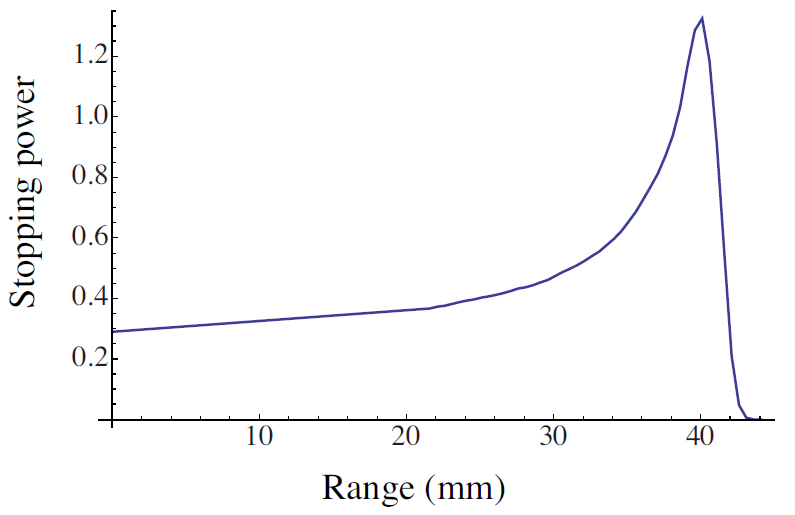
\includegraphics[scale=.25]{bragg.png}
    %\caption{Illustration of the bragg curve for charged particles. Picture from \cite{inbook}}
    %\label{fig:braggcurve}
%\end{figure}



\section{Radioactive decay}
\label{sec:Radioactivedecay}

- what is it
 
\section{Decay modes}
\label{sec:decaymodes}

-why are these usefull for nuclear medicine (therapy and diagnstics)


\subsection{$\beta$-decay}

Decay by $\beta$ can happen by $\beta$-, EC (see auger electrons) or $\beta$+ decay.\\
$\beta$-:
\begin{equation}
n \rightarrow p + e^- + \bar{\nu_e} 
\end{equation}\\
$\beta+$:
\begin{equation}
p \rightarrow n + e^+ + \nu_e
\end{equation}\\
For therapy, $e^-$ will travel longer in a medium than $e^+$ (will annihilate fast).\textcolor{red}{WHY?} $e^-$ will ionize matter on its path and we want to take advantage of that. Therefore, it is $\beta$- decay we are interested in when we treat a patient. $\beta$+ decay are used in diagnostic. If we want to take a picture of the biological activity in a patient, $e^+$ is the source of interest for usage of PET scans, which I will discuss in section 4.1.\\
\\
Compared to $\alpha$ particles, $\beta$ particles travels a lot further and creates less ionization to the surrounding medium on its path. This is important when the biological effect matters. There are however, difference in the range of various of isotopes that undergo $\beta$ decay. Short range $\beta$-particle emitters have a relatively short range, a couple of $\mu m$, in tissue that is suitable for treatment of small tumor metastases%\cite{nuclearchem}. 
The $\beta$-emitters with long range in tissue can penetrate with an average of more than 2 mm and can be used to treat i.e. rheumatoid arthritis, which is an autoimmune disorder that often affect joints.\\
\\
The energy of $\beta$ particles are not distinct, but rather more spread out in a spectrum.

%\begin{figure}[h!]
   % \centering
    %\includegraphics[scale=0.4]{betadecay.png}
    %\caption{A typical illustration of the energyspectra for beta decay. From \cite{medical}}
    %\label{fig:beta_decay_energyspec}
%\end{figure}

The spectrum in figure %\ref{fig:beta_decay_energyspec} 
shows how the energy are divided between the electron and the anti neutrino. The electrons of beta particles will interact with the surrounding electrons by dismissing the it from its orbit and producing a ion pair or cause excitation. Since the amount of damage tissue is related to LET and $\beta$ particles penetrates further in to a medium than $\alpha$ particles, $\beta$ particles has lower LET than $\alpha$ does. Exposure to $\beta$ results therefore in less damage.\\
\\
$^{90}Y$ is one popular long range isotope used in therapy, it has a mean range of 3.900 $\mu m$ and an average energy of 935 KeV%\cite{nuclearchem}
, while a widely used short range beta emitter is $^{131}I$. It has a mean range of 910 $\mu m$ and an average energy of 182 KeV%\cite{nuclearchem}.
 The energy will vary from almost zero to the maximum energy, and the average energy is approximately one third of the maximum energy. For therapy, the mean energy dependent mean and maximum range in tissue for beta emitters. 
\\
\\

\subsection{Electron capture, Internal convention and Auger electrons}

When low-energy X-ray photons collides with an atom and electron from the inner shell can get ejected. If the nucleus has too many protons, the electron can be captured by the nucleus where the electron and a proton turns into a neutron. This is called electron capture (EC). When this happens, there will be an empty spot in the K shell which one of the electrons in the L shell will try to fill. There will therefore be a vacancy in the L shell. This process releases an energy of $E_K - E_{L}$ and can be transferred to another electron in the L shell, resulting in ejecting it from the atom. This electron is called auger electron. It is a low energy electron that will have a kinetic energy of $T = E_k - E_{L1} - E_{L2,3}$ \cite{medical}, where $E_k - E_{L1}$ is the difference in binding energy. It has a short range and will deposit all of its energy in a highly localized site. The distance the auger electrons travels from <0.5 $\mu$m to a few nm in biological tissue \cite{augerelectrons}, it follows high LET and will therefor do a lot of damage to the DNA and other important structure in the cell nucleus that are important for the cell to live. Auger electrons are highly effective for killing these structure and breakage of double DNA strands due to its energy deposit in a short distance (see figure \ref{fig:auger}).\\
%\begin{figure}[h!]
%\centering
%\begin{subfigure}{.43\textwidth}
  %\centering
  %\includegraphics[width=.7\linewidth]{1200px-Auger_Process.jpg}
  %\caption{Illustration of emission of an auger electron, illustration from Wikipedia}
  %\label{subfig:augerlevel}
%\end{subfigure}%
%\begin{subfigure}{.43\textwidth}
  %\centering
  %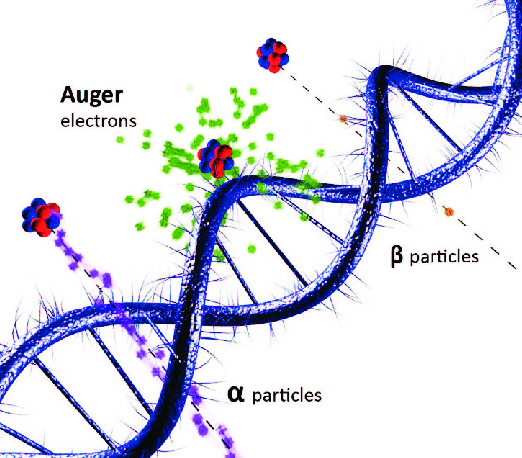
\includegraphics[width=.7\linewidth]{auger.png}
  %\caption{Range of auger electron compared to $\alpha$ and $\beta$ particles, taken from \cite{auger}}
  %\label{subfig:DNA}
%\end{subfigure}
%\caption{A description of auger electron}
%\label{fig:auger}
%\end{figure}
\noindent
\\
One other way auger electrons are created is due to the effect of internal conversion (IC). This is when an electron get knocked out of the inner shell and one other electron from a higher orbital jumps down to the inner shell. In this process energy gets realised by photons which can knock out an electron from the outer shell, the auger electron. 
\\
\\


\subsection{$\gamma$-decay and X-rays}

\textbf{$\gamma$ and X-rays}\\
\\
\noindent
Emission of $\gamma$-rays are usually a product from the radioactive decay of atomic nuclei. If the nucleus is left in an excited state, it will de-excite by either emit a photon.\cite{nuclearchem}. $\gamma$ decay are described as $$^{A}_{Z}X^* \rightarrow ^{A}_ZX + \gamma$$
where the excitation energy is transferred to a $\gamma$ photon plus the recoil energy.\\
\\
If the notation includes a "m" $$^{Am}_ZX \rightarrow ^{A}_ZX + \gamma$$
in that case, the nucleus is in an isomer state where it is long-lived $(T_{1/2} < 1 \mu s)$ in an excited state\cite{nuclearchem}. The transition will then be described as an isometric transition (IT).\\
\\
Competing with $\gamma$-ray emission, internal conversion (IC) is a way for the nucleus to de-excite. It will electromagnetically interact with a shell electron witch leads to emitting of the orbiting electron\cite{toxicology}.\\
\\
\\  
X-rays, as $\gamma$-rays, are electromagnetic radiation. The difference is that X-rays has its origin outside of the nucleus. When X-rays and $\gamma$ penetrates a medium it can create different effects in the body by ionization.
Photoelectric effect, Compton effect and pair production. \\
\\
\%begin{figure}[h!]
   % \centering
    %\includegraphics[width=190]{photoelectric_cross.png}
    %\caption{Cross section for photoelectric effect, Compton scattering and pair production. Taken from \cite{photoelectric_cross}}
    %\label{fig:photo-compton-pair}
%\end{figure}
\\
The photoelectric effect happens when a nucleus absorbs the incoming photon. The energy absorbed will be used to ejected an orbiting electron from the atom. This electron is called a photoelectron\cite{nuclearchem}. The electron cannot be emitted if the incoming photon energy is lower than the binding energy of the shell to the electron. The energy of the electron emitted is then $E_e = hv - E_b$. The probability of photoelectric effect happens is measured as the cross section 
$$\sigma = constant \cdot \frac{Z^n}{E^3}$$
where n is equal to 4 or 5\cite{Radiological_physics}. The photoelectric effect will increase with the atomic number and by that reason we are using lead (Z=82) as shielding for gamma radiation.\\ 
\\
Compton effect is scattering of a photon due to an electron. When an incident photon interacts with an atomic or free electron, it will bend from its original path with an angle $\theta$. The electron are then being emitted with an angle of $\phi$.\\
The energy is shared between the emitted electron and the photon, where the incident photon will transfer some of its energy to the electron. The final photon energy is $$h\nu' = \frac{h\nu}{1 + \frac{h\nu}{m_ec^2} (1-cos\theta)}$$
The atomic cross section is $$\sigma_a = Z \sigma_e$$ where $\sigma_e$ is the electronic cross section, assuming a free electron\cite{nuclearchem}.\\
\\
The last main effect is pair production. The incoming photon disappears, and spontaneously turns into an electron-positron pair. This can only happen if the energy of the photon is greater than the total rest mass of an positron-electron pair, 1.022 MeV. Since X-rays and $\gamma$ can penetrate long distances without ionizing the medium, emerges from the body and has a low LET, they are at good use for diagnostic of a patient with different imaging technique. \\
The cross section of pair is production is dependent on $Z^2$ .
\\
\\
Figure \ref{fig:photo-compton-pair} shows how the three main interaction of a photon is dependent on energy. For lower energies it is clear that the photoelectric effect is dominant, pair production is more probable to happen in higher energies.\\


\section{Theranostic}
\label{sec:theranostic}




% ----------------------------------------------------------------------------------------------------------------------
% ----------------------------------------------------------------------------------------------------------------------

\chapter{Cu64,67} 
\label{ch: mywork}

\epigraph{\itshape ``- The idea that everyone is supposed to buy into stuff without questioning it, is the reason why we are 51 year old 16 year olds.\\ 
- Dude, I agree. "}{--- \textup{Joe Rogan and Duncan Trussel}}


\section{what can we do to make the nuclear medicine better?}
\label{sec: betterwork}

-medical prespecctive: we wan to introduce a new theragnostic pairs to use in hospitals\\
- how wonderful Cu64,67 are\\
-- properties\\
-- papers\\
-- better than a lot of the studff we are already using\\
-- motivation for my work\\
---- can adjust ratio for 64,67 Cu by tuning the energy of the beam\\



\subsection{My motivation}
\label{sec: my_motivation}




\subsection{Physics motivation}
\label{sec: physics_motivation}

- cu64,67 are amazin but now, we have not a good way for making them. tell about my way of create them\\
-- deuterium breakup (n,-) way\\
-- how we are doing it\\


% ----------------------------------------------------------------------------------------------------------------------

% ----------------------------------------------------------------------------------------------------------------------

\chapter{The experiment}
\label{ch: experiment}

In this theses we wanted to study the $^{nat}Zn(n,x)^{64,67}Cu$ reaction. 
In the following chapter, the experiment in itself is being discussed. Sections 4.1.1, 4.1.2 and 4.1.3 describes the 88-Inch cyclotron used int the experiment, the deuterium breakup process and how the targets were stacked together before being irradiated.


\section{The experimental setup}
\label{sec: setup}

The experiment was preformed on August 2018 at the Lawrence Berkeley National Laboratory where six targets were irradiated with a neutron beam. The beam had to be tuned such that it didn't have a lot of angular distribution before it hits the targets. 

\textcolor{red}{Incert pic of the foils here!}
\\
\\
The targets were placed in a metallic box, see figure \ref{fig:target_stack}, and then placed in a tube that were sealed with vacuum. 

\begin{figure} [h]
   \centering
   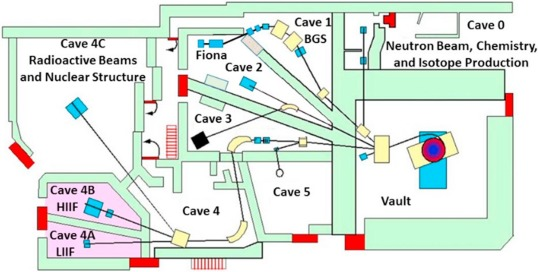
\includegraphics[scale=1.2]{88-inch_cyclotrone.jpg}
   \caption{Map over the 88-inch cyclotorne at Lawrence Berkeley National Laboratory\textcolor{red}{FROM?}}
   \label{fig:88-inc_cyclotron}
\end{figure}

- tuning of beam

\subsection{Cyclotron}
\label{sec: cyclotron}

Being one of the first cyclotrons used to produce medical isotopes, the Berkeley lab is still used to produce radionuclides that are a part of the research in the medical industry. Lawrence national laboratory is located in the hills, directly over the university of California at Berkeley overlooking San Francisco bay.\\
\\
The 88-Inch cyclotron is used in research on varies of fields including astrophysics and nuclear structure. The accelerator is a 300-ton, K = 140 sector-focused cyclotron with the ability to run with both heavy- and light-ions. The facility of the cyclotron is shown in figure \ref{fig:88-inc_cyclotron}, it mainly has five experimental caves where cave 0 is the one used for neutron beams and isotope production. The cyclotron can accelerate ions up to 70??? MeV  ...
\\
\\
- k-value (descuss energies for hospital cyclotrons and what energies for Cu64,67), what is it, how does it work\\
- no more than a page or two (look at other theses o se how deep you should go)

\subsection{Deuterium breakup prosess}
\label{sec: D_breakup}

Deuterium break up can be done on any material, but natural beryllium a dense medium that has the quality as a good conductor of heat, it is stable and it is impossible to produce a radioactive activation product using deuterium. There is no excited states in deuterium [https://www.nndc.bnl.gov/ensdf/EnsdfDispatcherServlet] and if we give it energy it will break up into a neutron and a proton.
\\
\\
- and how it is usefull for creating neutrons (brought energy spectrum that we can tune in terms of energy, inntense neutron source (makes a lot of neutrons) focused beam of neutrons \\
- moulders paper and other



\subsection{Stack design}
\label{sec: stack_design}

A specific design of the targets were used to make sure that the cross section for each target could be measured for the different energies we radiated the targets with. Five different targets, Al, In, Y, Zn, and Zr, were made into small “packings” using kapton tape to tightly seal them( see figure \ref{fig:target_design}), \textcolor{red}{ bruker dette også til å hinde contamination siden targetset kan være sjør og unngå spredning av løst radiaktivt stoff. }
\begin{figure} [h]
   \centering
   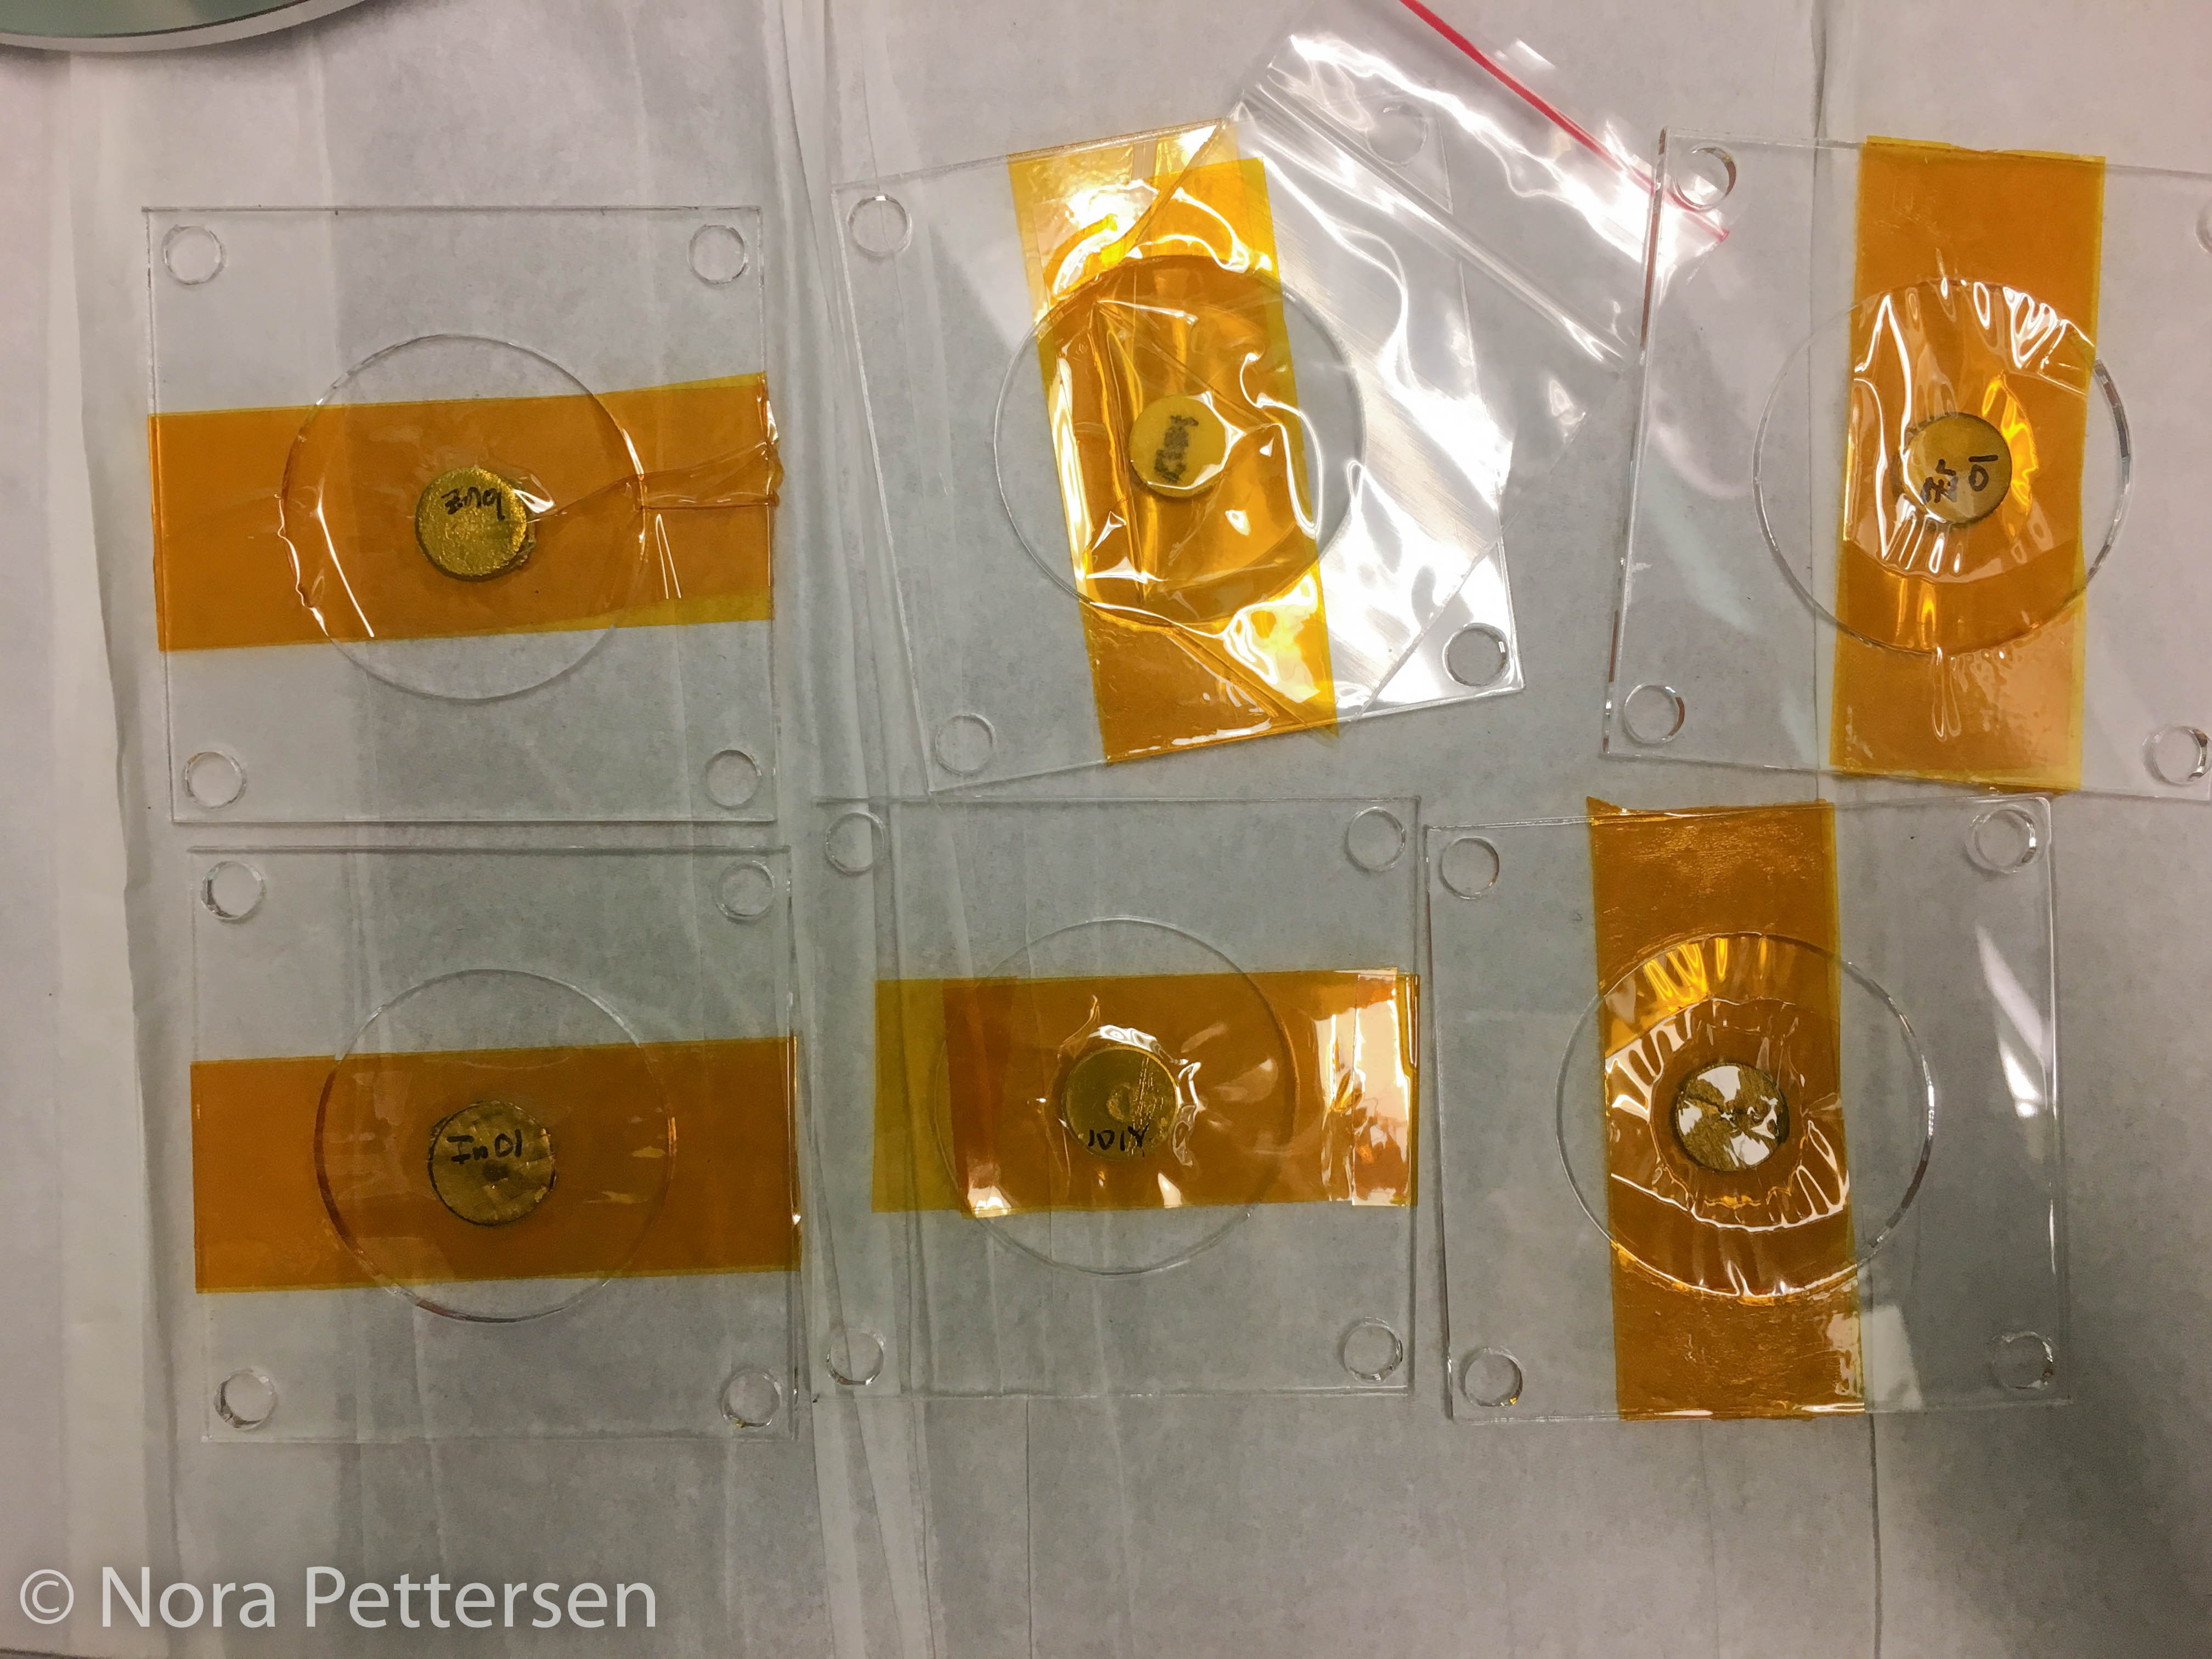
\includegraphics[scale=.2]{packs-1.JPG}
   \caption{Picture of how the targets were sealed before irradiation}
   \label{fig:target_design}
\end{figure}
\\
\noindent
The kapton contains polymer carbon, hydrogen and oxygen but the sticky part of the tape are made from silicone. For each target we measured their wight, thickness and length \textcolor{red}{Using what?} to calculate the uncertainty of each target. The targets were attached to a plastic frame and were placed in the end of a metallic \textcolor{red}{box made of?} where we wanted the targets to be 10 cm from the Br disk, the targets were held in place by a spring between them and the disk in front. 
\begin{figure} [h]
   \centering
   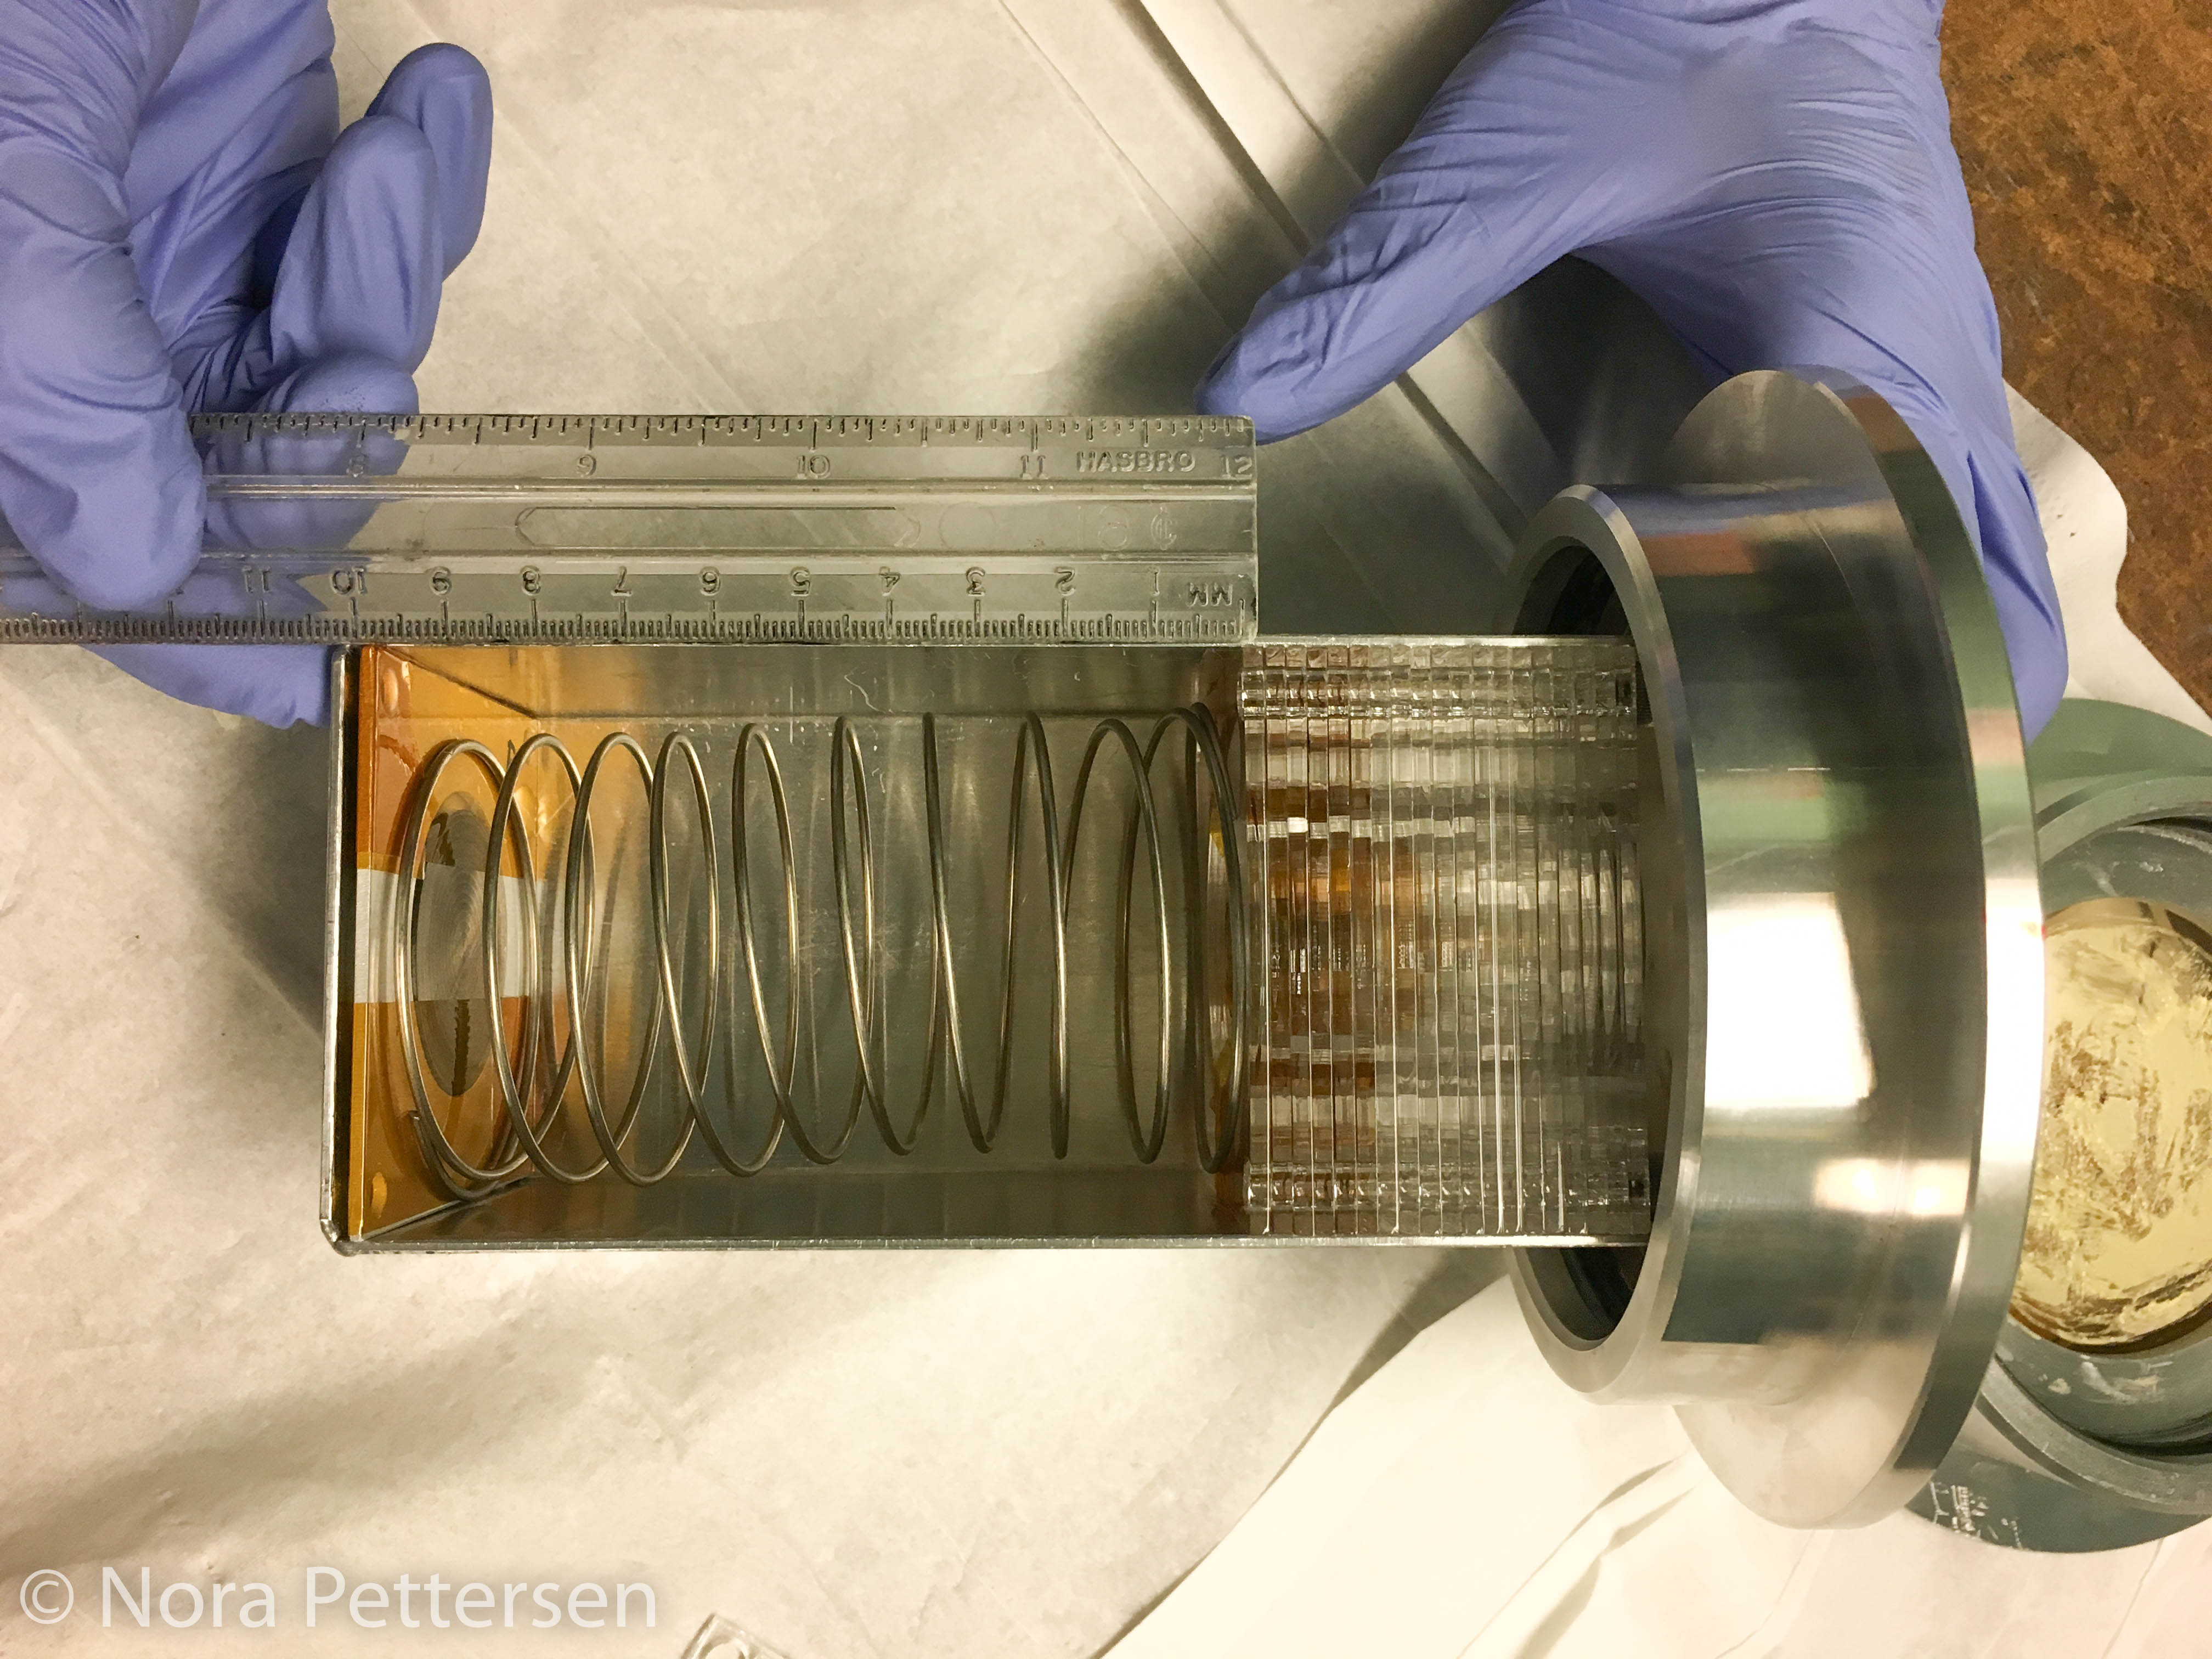
\includegraphics[scale=.2]{target_stack-1.JPG}
   \caption{Picture of how the targets were placed in the metallic box before irradiation}
   \label{fig:target_stack}
\end{figure}
\\
\noindent
The metallic box was then placed in the beamline by inserting it into a vacuumous tube. The vacuum was there to prevent the beam to hit air molecules and to make the beamline as straight as possible, such that more of the beam would be able to hit the targets. The radiation of the targets were on for approximately \textcolor{red}{12 hours?} for both 16 MeV and 33 MeV. 
\cite{E.Lawrence}


- photos and stuff\\
- monitor foils



\section{Radiation}
\label{sec:radiation}

- how long time\\
- beam current\\
- beam monitor to meassure the  \\
-- plot the beam current  as a function of time to justefy thet we can make the math that we do


\subsection{Counting}
\label{sec:counting}

- after each radiation, we removed the foils to the counting room (how long did this take?) hvor lang ti tok det før vi begynte å telle etter EOB?

\section{Gamma spectroscopy}
\label{sec: gamma_spectro}

- Detector\\
-- forklare hvor dypt jeg skal gå inn i physics (doping, n-p junktion)\\
-- pari production, comptopn og photoelectric effect


\subsection{Gamma spectra}
\label{sec: gamma_spectra}

- deadtime, og alt det der

\subsection{Calibrating}
\label{sec: calibrating}

- detectror efficincy\\
- curves at different position


% ----------------------------------------------------------------------------------------------------------------------
% ----------------------------------------------------------------------------------------------------------------------

\chapter{Analyse}
\label{ch:analyse}

\epigraph{\itshape ``If you ever start thinking too seriously, just remember that we are talking monkeys on an organic spaceship flying through the universe"}{--- \textup{Joe Rogan}}



\section{Fitz peak}
\label{sec:fitz_peak}

- Data to activity ( the math). Peak counts to activity\\
- i - Aktivity to A$\_$EOB\\
- Production physics (Analyse eller Resultater?) - how we calculate cross-sectrtion, the work with john to use the monitor data to neutron fluxes that I’m going to use for calculate the cross section for my isotopes



\subsection{Regression prosess}


\section{Priduction physics}
\label{sec: prod_physics}



% ----------------------------------------------------------------------------------------------------------------------% ----------------------------------------------------------------------------------------------------------------------

\chapter{Results and dscussion} 
\label{ch: res_and_discussion}
- Cross sections for all the isotopes\\
- experimentall data with the data that has been meassured so fare


\section{TALYS}
\label{sec: talys}


- tolking av resultat. Hvilke energier er best i forhold til hva vi ser?\\
- Verdien av dette i fremtiden?\\
- how can we  desien target for å kunne produsere mer Cu67. hvilke cyclotrons can we use for that? 




% ----------------------------------------------------------------------------------------------------------------------% ----------------------------------------------------------------------------------------------------------------------




\chapter{Summary and outlook}
\label{sum_and_outlook}
\citep{Prasad1971a}
\section{Future work}
\label{sec: future_work}


\epigraph{\itshape quote}{--- \textup by }

% ----------------------------------------------------------------------------------------------------------------------% ----------------------------------------------------------------------------------------------------------------------

%\begin{appendices}
%\chapter{Some Appendix}
%The...

%\blindtext


%\chapter{Some other appendix...}
%\blindtext

%\end{appendices}


%\bibliographystyle{unsrtnat}
%\bibliographystyle{mybibstyle} %my own bibstyle to set first names to one letter + unsrtnat
\bibliographystyle{IEEEtran}
%\bibliography{library.bib}

%\bibliography{/Users/ikkullma/Documents/MendeleyDesktop/Oslo_Method.bib,web_references.bib,other_ref.bib,/Users/ikkullma/Documents/MendeleyDesktop/GeneralNuclearPhysics.bib,/Users/ikkullma/Documents/MendeleyDesktop/NuclearAstro.bib}

%change the user...
\bibliography{/Users/Nora/Documents/UiO/Masteroppgaven/Oppgaven/library.bib}


\end{document}